\subsection{A generic asynchronous implementation}

Let us finally consider a last aspect of asynchronous computation, i.e. not the fact that we want to simulate a continuous system in an asynchronous way, but the fact that we want to simulate a system {\em intrinsically asynchronous} in a sequential or distributed computational device.  This covers two fundamental aspects.  On one hand, each unit has a local clock, so the state evolution depends entirely on the occurrence of asynchronous mechanisms over time.  This means there are delays between units, with unpredictable exact values.  On the other hand, there is another semantics related to anachronism, i.e. the fact that information associated to input and output is defined by both a value and the time at which the value is issued.  In other words, the information is defined through temporal events.

Concerning biologically plausible models, the event-driven computation scheme has been mainly developed for spiking neuron models.  Such models are not addressed here \footnote{see \cite{Gerstner:2002} for an introduction and \cite{Cessac:2008,Cessac:2010} for a recent theoretical analysis and general discussion in link with these aspects}. Nevertheless, this scheme could be certainly extended at a more mesoscopic level, as that of cortical columns, modeled by dynamical neural fields, as developed here. The dedicated simulation tool is an event-based neuron simulation kernel as proposed by, e.g., \cite{Rochel:2003} based on the well-known Discrete Event System Specification (DEVS) framework (for a comparative review see \cite{Brette:2007}), very easy to simulate on a single processor.\\

Very concretely, each unit is defined by three functions: (i) The next event function provides an estimation of a lower-bound of the future time, where the next event time is going to be fired. (ii) Two update functions define how the unit update its state when either its own internal event, or another incoming external event is issued. The DEVS allows to show that given this specification, a complete asynchronous system can be simulated, using a simple calendar queue of events, on any device (see, e.g., \cite{Cessac:2009} for details). This allows not only to simulate asynchronous calculations on a centralized system, but also to {\em mix} both kinds of implementation. 

In brief, we propose to not only use event-based unit simulation at the microscopic level, targeting spiking-neurons, but also at the mesoscopic level, modeling the emergence of temporal events (synchronization or more complex mesoscopic spiking patterns, dynamic change triggering, etc..).

\subsubsection*{An illustrative example}

Let us instantiate this general discussion, through an illustrative example. In a recent work \cite{Rougier:2006} a model has been designed that performs global competition, only using local connections, with diffusion of the inhibition throughout the network. This is far quicker to have a few local interactions when computing activity within the network and this makes the model a real candidate for distributed computations.
We have re-implemented this mechanism considering asynchronous sampling via a minimal event-based simulation 
kernel\footnote{Code available at {\tt http://enas.gforge.inria.fr},
while {\tt EnaS} is the general purpose large-scale event-based multi-scale simulator at the edge of the state of the art.},
which obviously works since the system is still contracting when using asynchronous sampling, as discussed previously. 
This has been numerically experimented, as shown in Fig.~\ref{fig:bump}, 
with the obvious heuristic to have the local sampling period roughly proportional to the state value variation (parsimonious principle),
with a strong robustness with respect to the related parameters (modifying the asynchronous paradigms changes the transitional values, slightly influences  the convergence speed, but does not modify the final result).

This numerical result corresponds to trivial implementation of~(\ref{eq:DNF-solution}), so that the convergence is really obtained thanks to asynchronous paradigm. We have numerically verified on this simulated example that we could approximate the true solution at any precision (which was obviously expected anyway). Though this is not informative to report in details, we have been able to reproduce all qualitative DNF input/output functions ({\em filtering} of the output bump shape, {\em selection} of the output bump among several input bumps, {\em tracking} of a moving input bump at the output level, {\em remanence} of the output bump after the partial or total suppression of the input bump, see \cite{Alexandre:2009} for details). We have been able to verify that providing that~(\ref{eq:convergence}) is verified, the computation was guaranteed in all observed cases while if far away from this bound, it is expected to fail. It is however still an open point to verify whether this bound is numerically a thick one, in all interesting case.
%%
\begin{figure}[ht]
\centerline{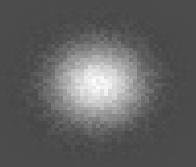
\includegraphics[width=0.25\textwidth,height=0.25\textwidth]{Chapitres/PublicationsSample/Revue/fig2a.jpeg}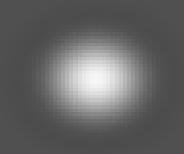
\includegraphics[width=0.25\textwidth,height=0.25\textwidth]{Chapitres/PublicationsSample/Revue/fig2b.jpeg}}
 \caption{An example of asynchronous sampling of such maps (event-based implementation), applying convergence criteria derived here.  We have numerically verified the conjecture that the present results apply when using asynchronous sampling.  {\em Left view}: intermediate result, the fact asynchronous sampling yields randomization is visible.  {\em Right view}: final result, after convergence.}
\label{fig:bump} 
\end{figure}
%%
Though this is only a preliminary result that opens large perspectives on new asynchronous paradigms for discrete neural field implementations.
